\documentclass[a4paper,10pt]{article}
\usepackage[latin1]{inputenc}
%\usepackage{color}
%\usepackage{colortbl}
%\usepackage{amstext}
\usepackage{amsmath}
%\usepackage{graphicx}
\usepackage{pgfplotstable}

\makeatletter
\makeatother

\begin{document}

\title{Gekoppelte Pendel}
\author{Andreas Zuber, Florian Schnider}

\maketitle

\section{Einleitung}
In diesem Versuch untersuchen wir ein gekoppeltes Pendel. Die Apparatur besteht
aus Zwei Pendel die mittels einer Feder verbunden sind.

\subsection{Ziel des Versuches}
Zeil des Versuchs ist es die beiden Pendel in verschiedenen Konfigurationen zu vermessen und die Messresultate
mit den Werten aus der Theorie zu vergleichen.

\subsection{Versuchsaufbau}
% - Skizze
% - Ger�tenummern
% ...
\begin{figure}[htp]
 \centering
 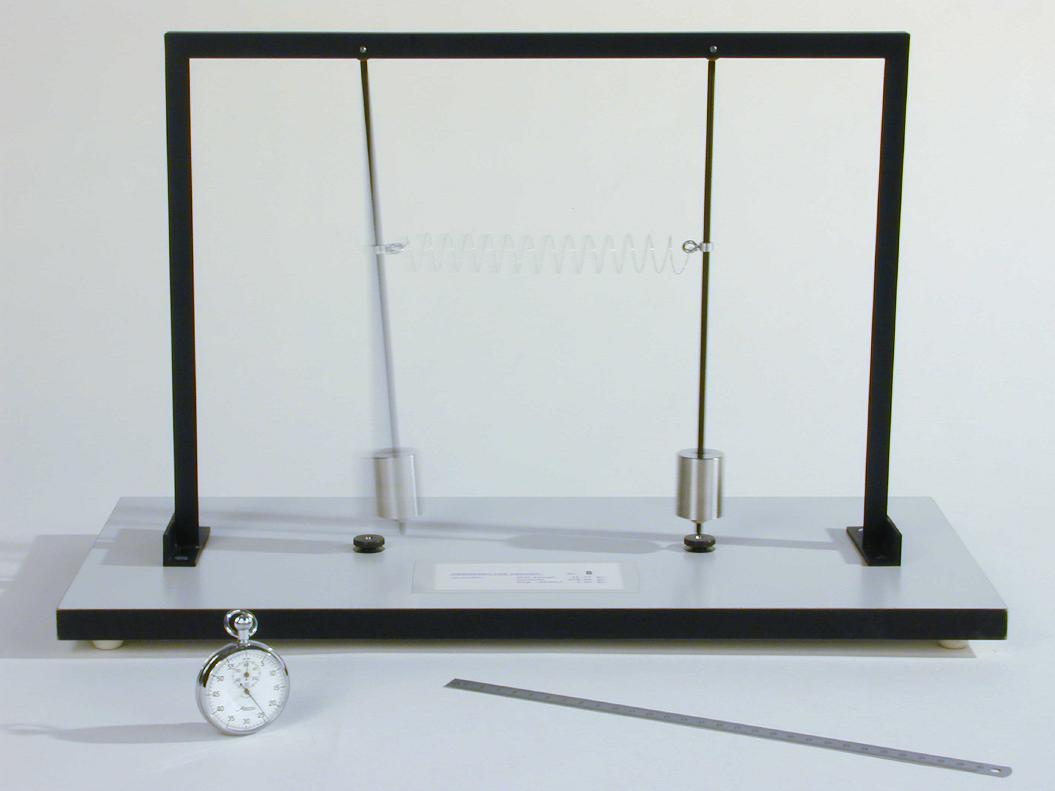
\includegraphics[scale=0.3]{./versuch_03_gekoppelte_pendel_versuchsaufbau.jpeg}
 \caption{Versuchsanordnung}
\end{figure}


\begin{itemize}
 \item Apparatur mit gekoppeltem Pendel Nr. 5 bestehend aus Gewicht, Mutter und Stab
 \item Kopplungsfeder
 \item Massstab
 \item Uhr
\end{itemize}

Werte zum Versuchsaufbau:
\begin{itemize}
 \item $m = 214,15g$ : Masse des Gewichts
 \item $m' = 21,37g$ : Masse des Pendelschafts
 \item $m_r = 2,00g$ : Masse der Reguliermutter
 \item $d = 264mm$ : Distanz Achsenmittelpunkt bis Gewichtsmittelpunkt 
\end{itemize}

\begin{figure}[htp]
 \centering
 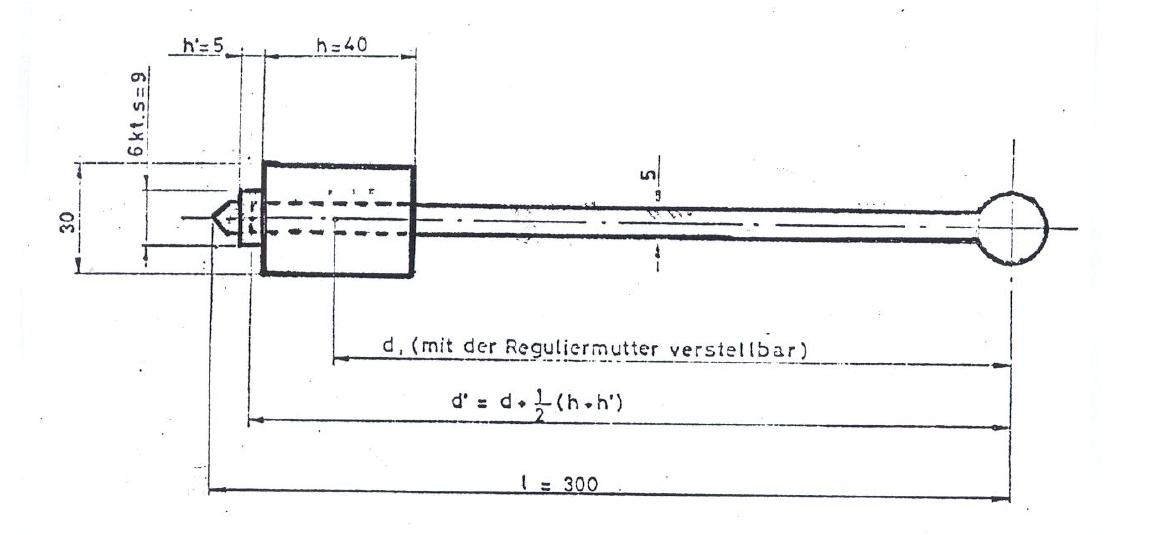
\includegraphics[scale=0.3]{./versuch_03_gekoppelte_pendel_pendel.jpeg}
 \caption{Dimensionen des Pendels}
\end{figure}

\section{Theorie}
% - Zusammenfassung und Zusammenstellung der f�r die Auswertungben�tigten Formeln
Die Schwingungsdauer f�r die verschiedenen F�lle die wir im Experiment messen k�nnen 
theoretisch berechnet werden. Die Herleitungen der Formeln befinden sich im Script\cite{Script}

\begin{itemize}
 \item $\varphi_1, \varphi_2$ : Auslenkung der Pendel
 \item $\phi$ : Auslenkung zur Zeit $t_0$
 \item $J$ : Tr�gheitsmoment des Pendels
 \item $D_g$ : Direktionsmoment
 \item $D_f$ : Kopplungsmoment
\end{itemize}

F�r alle F�lle gilt, die Startgeschwindigkeiten sind 0. $\frac{d\varphi_1}{dt}=0, \frac{d\varphi_2}{dt}=0$

\subsection{Fall 1: $\varphi_1=\phi, \varphi_2=\phi$}
Die Auslenkung der Beiden Pendel zur Zeit $t_0$ ist gleich und in gleicher Richtung. Die
Pendel schwingen somit auch in die selbe Richtung. Die Schwingungsdauer in dieser Konfigurationen
wird mit $\tau_\omega$ bezeichnet.

\begin{center}
\[\tau_\omega=2\pi\sqrt{\frac{J}{D_g}}\]
\end{center}

\subsection{Fall 2: $\varphi_1=\phi, \varphi_2=-\phi$}
Die Auslenkung der beiden Pendel zur Zeit $t_0$ ist gerade entgegengesetzt. Sie schwingen also
auch in entgegengesetzter Richtung. Die Schwingungsdauer in dieser Konfiguration wird mit
$\tau_\Omega$ bezeichnet.

\begin{center}
\[\tau_\Omega=2\pi\sqrt{\frac{J}{D_g+2D_f}}\]
\end{center}

\subsection{Fall 3: $\varphi_1=\phi, \varphi_2=0$}
In diesm Fall wird nur das erste Pendel ausgelenkt. Das zweite ruht in $\varphi_2=0$.
Die Schwingun eines Pendels in dieser Konfiguration wird mit $\tau$ bezeichnet.

W�rend nun das erste Pendel schwingt wird �ber die Feder die Schwingungsenergie langsam
auf das zweite Pendel �bertragen. Die Amplitude des ersten Pendels wird im laufe der Zeit
kleiner bis es ganz zum Stillstand kommt und s�mtliche Schwingungsenergie im zweiten Pendel
steckt. Nun kehrt sich der Prozess gerade um und die Schwingungsenergie fliesst wieder zur�ck
zum ersten Pendel. Diese Schwingung des Gesammtsystems nennt man Schwebung und ihre Schwingdauer
ist in diesem Fall von interesse und wird mit $T_s$ bezeichnet.

\begin{center}
\[\tau=\frac{4\pi}{\Omega+\omega}\]
\[T_s=\frac{2\pi}{\Omega-\omega}\]
\end{center}

\subsection{Direktions- und Koppungsmoment}
Das Direktions- und Kopplungsmoment kann berechnet werden wenn das Tr�gheitsmoment
bekannt ist und die jeweils relevante Schwingungsdauer.

\begin{center}
\[D_g=\frac{4\pi^2J}{\tau_\omega^2}\]
\[D_f=2\pi^2J(\frac{1}{\tau_\Omega^2}-\frac{1}{\tau_\omega^2})\]
\end{center}

\subsubsection{Dynamische bestimmung}
Das Direktions- und Kopplungsmoment kann auch statisch bestimmt werden. Dabei wird
das erste Pendel in eine Position $\phi_1$ ausgelenkt. Beim zweiten Pendel stellt sich
nun die Auslenkung $\phi_2$ ein.

\begin{center}
\[D_g=gl(m+\frac{m'}{2})\]
\[D_f=gl(m+\frac{m'}{2})\frac{\phi_1}{\phi_2-\phi_1}\]
\end{center}

\subsection{Kopplungsgrad}
Der Kopplungsgrad h�ngt von $D_f$ und $D_g$ ab. Er kann also sowohl aus den Schwingungszeiten
wie auch statisch aus den Auslenkungen bestimmt werden.

\begin{center}
\[k=\frac{\tau_\omega^2-\tau_\Omega^2}{\tau_\omega^2+\tau_\Omega^2}=\frac{\phi_1}{\phi_2}\]
\end{center}

\subsection{Tr�gheitsmoment}
Das Tr�gheitsmoment eines Pendels setzt sich aus den einzelnen Tr�gheitsmomenten seiner 
Komponenten zusammen.

\begin{itemize}
 \item $J_p$ : Tr�gheitsmoment eines Pendels
 \item $J_g$ : Tr�gheitsmoment des Gewichts
 \item $J_S$ : Tr�gheitsmoment des Schafts
 \item $J_R$ : Tr�gheitsmoment der Reguliermutter
\end{itemize}


\begin{center}
\[J_p=J_g+J_S+J_R\]
\[J_g=\frac{m}{12}(3(R^2+r^2)+h^2+12d^2)\]
\end{center}


\subsection{Fehlerrechnung}

\section{Messungen}
% - Alle Messwerte in �bersichtlichen Tabellen mit Mittelwerten und Fehlerangaben

\section{Diskussion}
% - Kommentare
% - Vergleich der Messwerte mit Theorie und Literaturwerten
% - Hinweis auf m�glich Fehlerquellen (besonders systematische Fehler)
% - Schwierigkeiten bei der Messung
% ...


\begin{thebibliography}{99}

\bibitem{Script} Anleitung zum Physikpraktikum, Praktikumsskript FS 2012, P. Wurz

\bibitem{Analysis} Skript zu Analysis I, C. Tretter

\end{thebibliography}

\end{document}